\documentclass[class=report, crop=false, 12pt,a4paper]{standalone}
\usepackage{enumitem}
\usepackage{multicol}
\usepackage{graphicx}
\usepackage{float}
\usepackage{amsmath}
\usepackage{amssymb}
\usepackage{mathtools}
\usepackage{siunitx}
\usepackage{commath}
\usepackage{array}
\usepackage{natbib}
\usepackage[a4paper,width=150mm,top=25mm,bottom=25mm]{geometry}
\setlength{\parindent}{0pt}
\begin{document}
\subsection*{Potential energy}
We know from everyday life that external loads of tension and compression produce very different responses in beams (not jus a change in the stress sign). This is due to the fact that tension and compression are associated with different behaviour in term of equilibrium.
\begin{figure}[H]
    \centering
    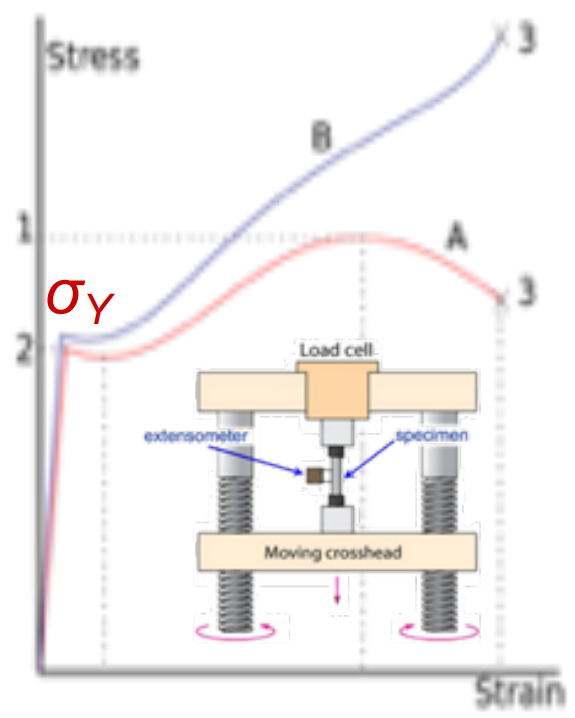
\includegraphics[width = 0.8\textwidth]{../img/diagram22.png}
    \caption{}
\end{figure}
\subsection*{Buckling}
This phenomenon, that produce the sudden bow of long struts, is known as instability or buckling, as the member is said to buckle. It is essential that for the design of safe structures we have to be able to predict if a member under compressive load would buckle.
\begin{figure}[H]
    \centering
    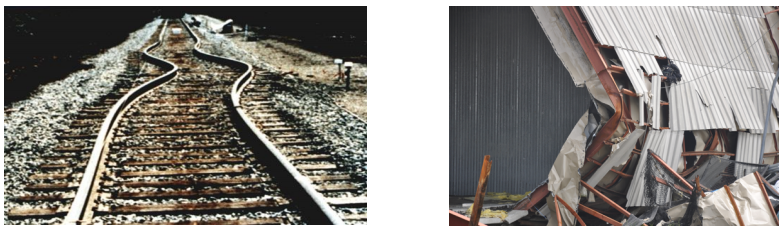
\includegraphics[width = 0.8\textwidth]{../img/diagram23.png}
    \caption{}
\end{figure}
\section{Euler's analysis of buckling}
\subsection{Euler buckling theory}
Assumptions:
\begin{itemize}
    \item The strut is ideal and perfectly straight when unloaded
    \item Axial load is applied at the centroid of cross-section
    \item The dimensions of the section are much smaller than the strut length
    \item All main assumptions of bending theory apply
    \item The beam material is perfectly homogeneous and isotropic
    \item The elastic limit is nowhere exceeded
    \item Young's Modulus for the material is the same in tension and compression
    \item Plane cross-sections remain plane before and after bending
    \item Every cross-section in the beam is symmetrical about the plane of bending
\end{itemize}
\begin{figure}[H]
    \centering
    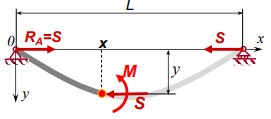
\includegraphics[width = 0.4\textwidth]{../img/diagram24.png}
    \caption{}
\end{figure}
Internal forces:
\begin{align}
    x) & \ P = - S\\
    X) & \ M = S \cdot y
\end{align}
From the theory of bending:
\begin{gather}
    \frac{\dif^2 y}{\dif x^2} = - \frac{1}{EI}M = -\frac{S}{EI}y\\
    \frac{\dif^2 y}{\dif x^2} + \frac{S}{EI}y = 0
\end{gather}
To solve a second order differential equation, we have to:
\begin{enumerate}
    \item find the complementary function $y_{CF}$
    \item find the particular integral $y_{PI}$
    \item the general solution is given by $y = y_{CF} + y_{PI}$
    \item find the particular solution using boundary conditions
\end{enumerate}
For differential equations in the form:
\begin{equation}
    \frac{\dif^2 y}{\dif x^2}+ \alpha^2 y = f(x)
\end{equation}
$y_{CF}$ has standard solution:
\begin{equation}
    y_{CF} = A\sin{\alpha x} + B\cos{\alpha x}
\end{equation}
Then, using substitution:
\begin{equation}
    \alpha^2 = \frac{S}{EI}
\end{equation}
This becomes:
\begin{equation}
    \frac{\dif^2 y}{\dif y^2} + \alpha^2 y = 0
\end{equation}
With standard solution:
\begin{equation}
    y_{CF} = A\sin{\alpha x} + B\cos{\alpha x}
\end{equation}
Since $f(x) = 0$, the particular integral is:
\begin{equation}
    y_{PI} = 0
\end{equation}
Therefore, the complementary function corresponds to the general solution:
\begin{equation}
    y = A\sin{\alpha x} + B\cos{\alpha x}
\end{equation}
Boundary conditions:
\begin{gather}
    \begin{cases}
        y(0) = 0\\
        y(L) = 0
    \end{cases}
\end{gather}
First boundary condition:
\begin{gather}
    y(0) = A\sin 0 + B\cos 0\\
    \therefore B = 0
\end{gather}
Our equation becomes:
\begin{equation}
    y = A\sin{\alpha x}
\end{equation}
Second boundary condition:
\begin{gather}
    y(L) = A\sin{\alpha L} = 0
\end{gather}
Equations accepts infinite solutions:
\begin{align}
    \begin{cases}
        A = 0\\
        \alpha L = n\pi \textrm{ with } n = 0,\, 1 ,\, 2\, , ...
    \end{cases}
\end{align}
Trivial solutions:
\begin{align}
    A = 0 \rightarrow y(x) &= 0 \textrm{ no buckling}\\
    \alpha L = 0 \rightarrow y(x) & = 0 \textrm{ no buckling}\\
    \alpha^2 = \frac{S}{EI} \rightarrow \alpha L &= \sqrt{\frac{S}{EI}}\cdot L = 0 \rightarrow \begin{cases}
        L = 0\\
        S = 0\\
        E = \infty\\
        I = \infty
    \end{cases}
\end{align}
Solutions of interest:
\begin{align}
    \textrm{Solution } \alpha L =\, & \pi \, \left(n=1\right)\\
    \rightarrow \, & y(x) = A\sin\left(\frac{\pi}{L}x\right)\\
    \alpha^2 = \frac{S}{EI} \rightarrow \alpha L =\, & \sqrt{\frac{S}{EI}}\cdot L = \pi
\end{align}
Critical load (mode 1):
\begin{equation}
    S_{cr} = \frac{\pi^2 EI}{L^2}
\end{equation}
\begin{figure}[H]
    \centering
    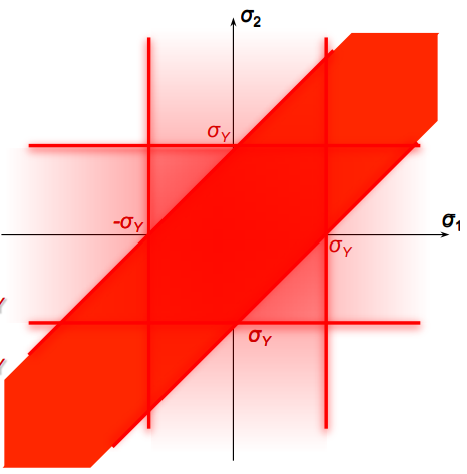
\includegraphics[width = 0.4\textwidth]{../img/diagram25.png}
    \caption{}
\end{figure}
Critical load (higher modes)
\begin{equation}
    S_{cr} = \frac{n^2 \pi^2 EI}{L^2}
\end{equation}
\begin{figure}[H]
    \centering
    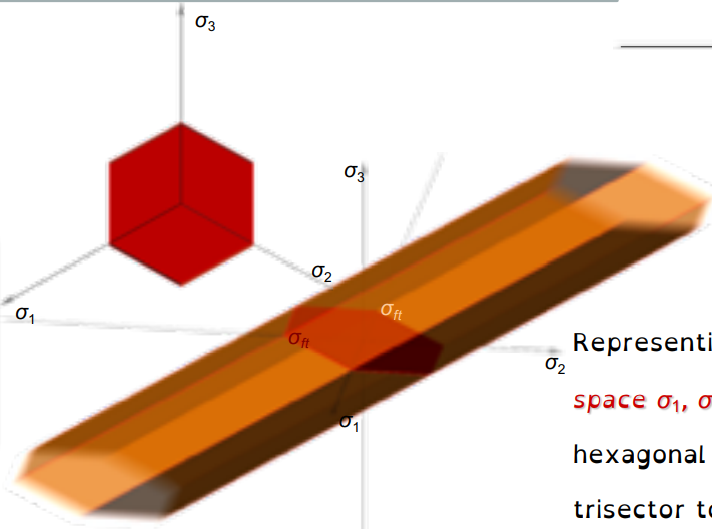
\includegraphics[width = 0.6\textwidth]{../img/diagram26.png}
    \caption{}
\end{figure}
\subsection{Buckling modes}
\begin{figure}[H]
    \centering
    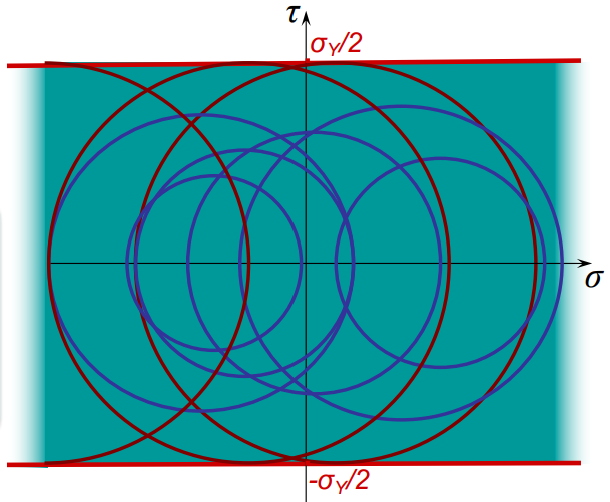
\includegraphics[width = 0.8\textwidth]{../img/diagram27.png}
    \caption{}
\end{figure}
The first buckling mode (n=1) is reached at the lowest critical load, and therefore is the one that occurs in normal conditions. Higher modes can be produced by applying external constrains at the points of contraflexure.
\subsection{Stress in buckling}
For the equilibrium of internal forces, stresses at each section will have to balance:
\begin{figure}[H]
    \centering
    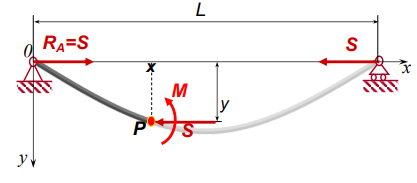
\includegraphics[width = 0.7\textwidth]{../img/diagram28.png}
    \caption{}
\end{figure}
Normal force contribution:
\begin{align}
    \sigma_x' = -\frac{S}{A}
\end{align}
Where $A$ is the area of the section.
\begin{figure}[H]
    \centering
    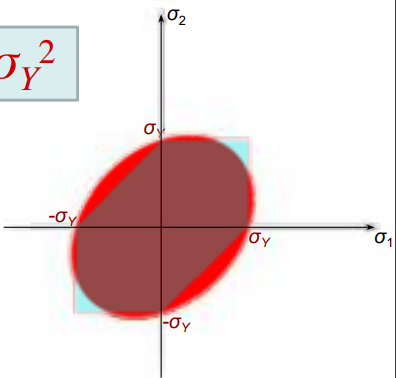
\includegraphics[width = 0.7\textwidth]{../img/diagram29.png}
    \caption{}
\end{figure}
Bending moment contribution:
\begin{align}
    \sigma_x'' = \frac{M}{I}h = \frac{Sh}{I}y
\end{align}
Where $I$ is the area of the section.
\begin{figure}[H]
    \centering
    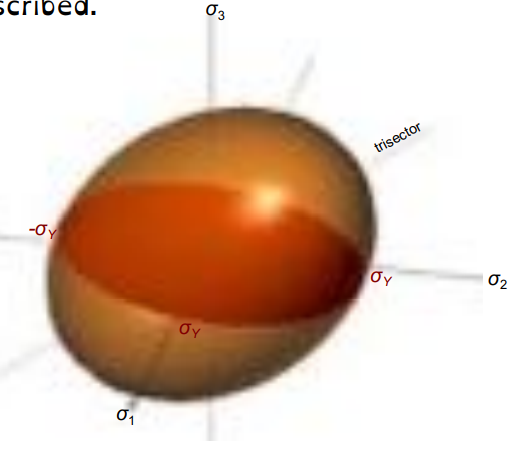
\includegraphics[width = 0.7\textwidth]{../img/diagram30.png}
    \caption{}
\end{figure}
\begin{align}
    \sigma_x = \sigma_x' + \sigma_x''= -\frac{S}{A} + \frac{Sh}{I}y = S\left(\frac{h}{I}y - \frac{1}{A}\right)
\end{align}
\subsection{Struts with other end conditions}
\begin{figure}[H]
    \centering
    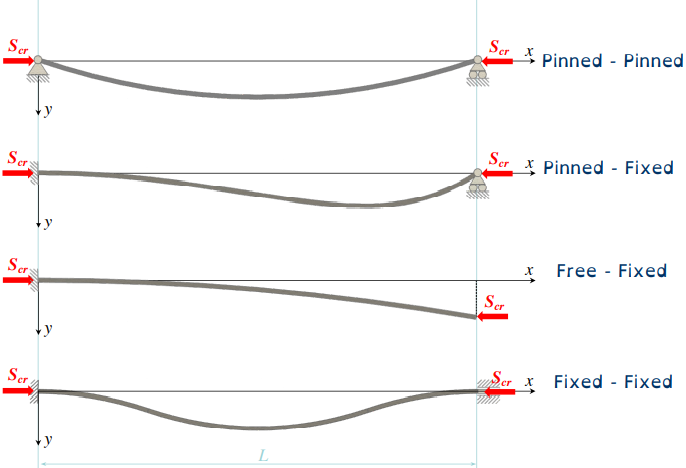
\includegraphics[width = 0.7\textwidth]{../img/diagram31.png}
    \caption{}
\end{figure}
\subsection{Effective length}
Expressions for the critical load for each end condition can be calculated adopting the same approach as for the pinned-pinned case. The form of expression is identical irrespective of the end conditions. 
\begin{align}
    S_{cr} = \frac{\pi^2 EI}{L^2_e}
\end{align}
Where $L_e$ is the \textbf{effective length}.
\begin{figure}[H]
    \centering
    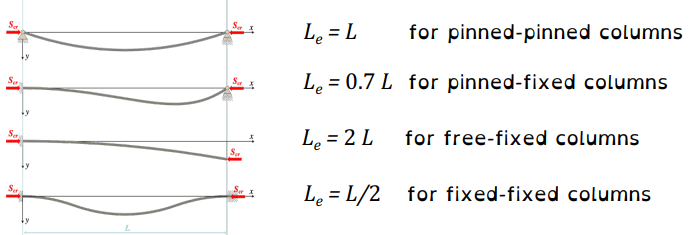
\includegraphics[width = 0.9\textwidth]{../img/diagram32.png}
    \caption{}
\end{figure}
\begin{figure}[H]
    \centering
    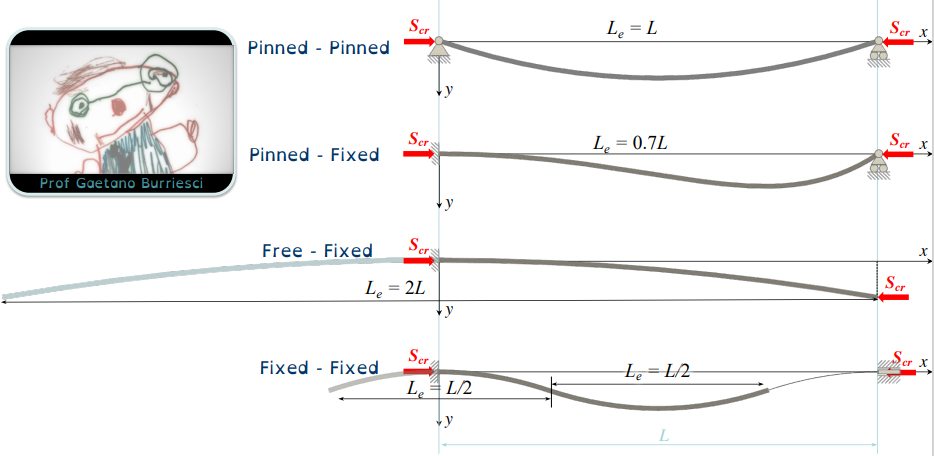
\includegraphics[width = 0.9\textwidth]{../img/diagram33.png}
    \caption{}
\end{figure}
\subsection{Design against buckling}
\begin{figure}[H]
    \centering
    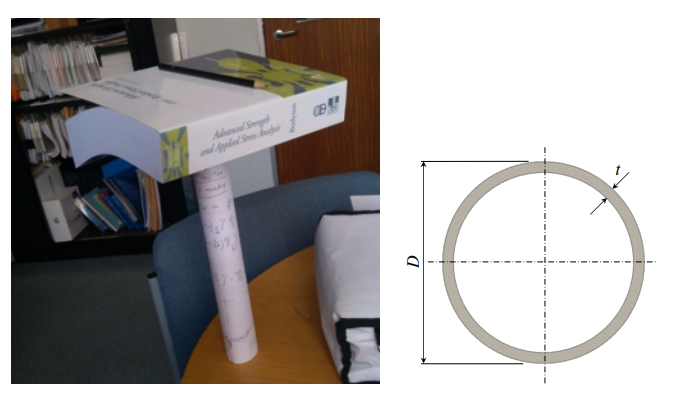
\includegraphics[width = 0.9\textwidth]{../img/diagram34.png}
    \caption{Hollow sections provide a greater critical load for a given cross-sectional area.}
\end{figure}
\begin{figure}[H]
    \centering
    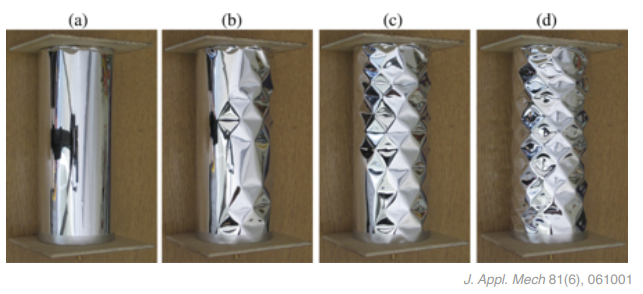
\includegraphics[width = 0.9\textwidth]{../img/diagram35.png}
    \caption{If the $\frac{D}{t}$ ration is too high, then local instability in the wall will occur.}
\end{figure}
Structural sections are often made to have a preferred failure plane: buckling occurs in the plane of least second moment of area of the cross-section. 
\begin{figure}[H]
    \centering
    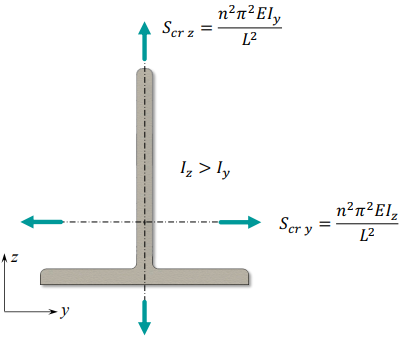
\includegraphics[width = 0.5\textwidth]{../img/diagram36.png}
    \caption{}
\end{figure}
Additional supports shorten the effective length of the column (structure has to buckle following higher critical loads modes).
\begin{figure}[H]
    \centering
    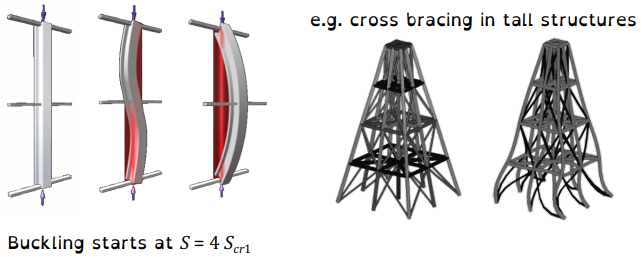
\includegraphics[width = 0.8\textwidth]{../img/diagram37.png}
    \caption{}
\end{figure}
\end{document}